%%%%%%%%%%%%%%%%%%%%%%%%%%%%%%%%%%%%%%%%%%%%%%%%%%%%%%%%%%%%%%%%%%%%%%%%%%%%%%%
% intro.tex: Introduction to the thesis
%%%%%%%%%%%%%%%%%%%%%%%%%%%%%%%%%%%%%%%%%%%%%%%%%%%%%%%%%%%%%%%%%%%%%%%%%%%%%%%%
\chapter{Introduction}
\label{intro_chapter}
%%%%%%%%%%%%%%%%%%%%%%%%%%%%%%%%%%%%%%%%%%%%%%%%%%%%%%%%%%%%%%%%%%%%%%%%%%%%%%%%

Kepler's laws of planetary motion, published over a period from 1609 to 1619, describe the motion of planetary orbits as ellipses about a central mass, predicting their orbital period and velocity based on the distance of the semi-major axis~\cite{kepler, russell}.
Shown by Isaac Newton in 1687~\cite{newton} to arise directly from his laws of motion and gravitation, Kepler's laws are well understood, extensively tested within our solar system, and, when applied to stellar orbits based on luminous matter in rotating galaxies, highly inconsistent with observation.

The first hint of a problem was found by Jan Oort in 1932, when he measured the velocities of stars in the solar neighborhood. 
Though later found to be inconsistent with modern measurements, Oort observed that the stars he measured were all moving faster than expected based on the visible mass distribution.
Later, Fritz Zwicky measured the velocity of stars in the Coma Cluster and in a 1937 paper~\cite{Zwicky} used the virial theorem to predict the total mass of the cluster, finding it to be around two orders of magnitude larger than expected from the cluster luminosity. 
Several other experiments observed similar effects over the following decades, which were generally attributed to light absorption within the galaxies or other systematic errors.

The first measurement of a galaxy rotation curve that agrees with modern observations was made in 1957 by Hendrik van de Hulst using the Dwingeloo 25 meter telescope~\cite{deHulst}, which confirmed earlier suspicions that the velocities did not match what was expected using only the luminous matter.
Later, a 1980 survey of 21 spiral galaxies lead by Vera Rubin~\cite{RubinSurvey} made precise measurements of the stellar velocity and verified the earlier measurements showing unexpectedly high orbital velocities, additionally finding that this excess velocity was present in \textit{all} galaxies surveyed, covering a wide range of luminosities and radii.

These unexpectedly large stellar velocities can potentially be explained through the presence of large amounts of additional mass, which would increase the gravitational attraction and produce similar increases in rotational velocity. 
The excess mass required for this explanation is not explicable solely through uncertainties in the masses of the stars themselves, as this would produce a multiplicative increase in the rotational velocity, while in data the distribution of velocity with distance from the galactic center has a fundamentally different shape than expected from only visible light.
In fact, the stellar velocities are seen to continue increasing up to the outermost stars, suggesting that this excess matter can extend some distance beyond the galaxies themselves. 
An example of a stellar rotation curve, along with a comparison of the observed velocity curve and what is expected from the visible light, is shown in \Cref{fig:rotCurve}.

Calculations of the necessary mass find that, if Newtonian gravity still holds, the excess matter must outweigh visible matter by a significant margin. 
Many theories have been presented to explain these observations, but one of the best motivated theories currently is that of some new dark matter particle, which would exist in great abundance throughout the universe and interact very feebly, if at all, with normal matter.
Particulate dark matter is largely favored due to several astronomical observations beyond direct measurement of rotation curves, including measurements of the cosmic microwave background, gravitational lensing, and simulations of galaxy structure formation and baryogenesis in the early universe.

\begin{figure}
   \centering
   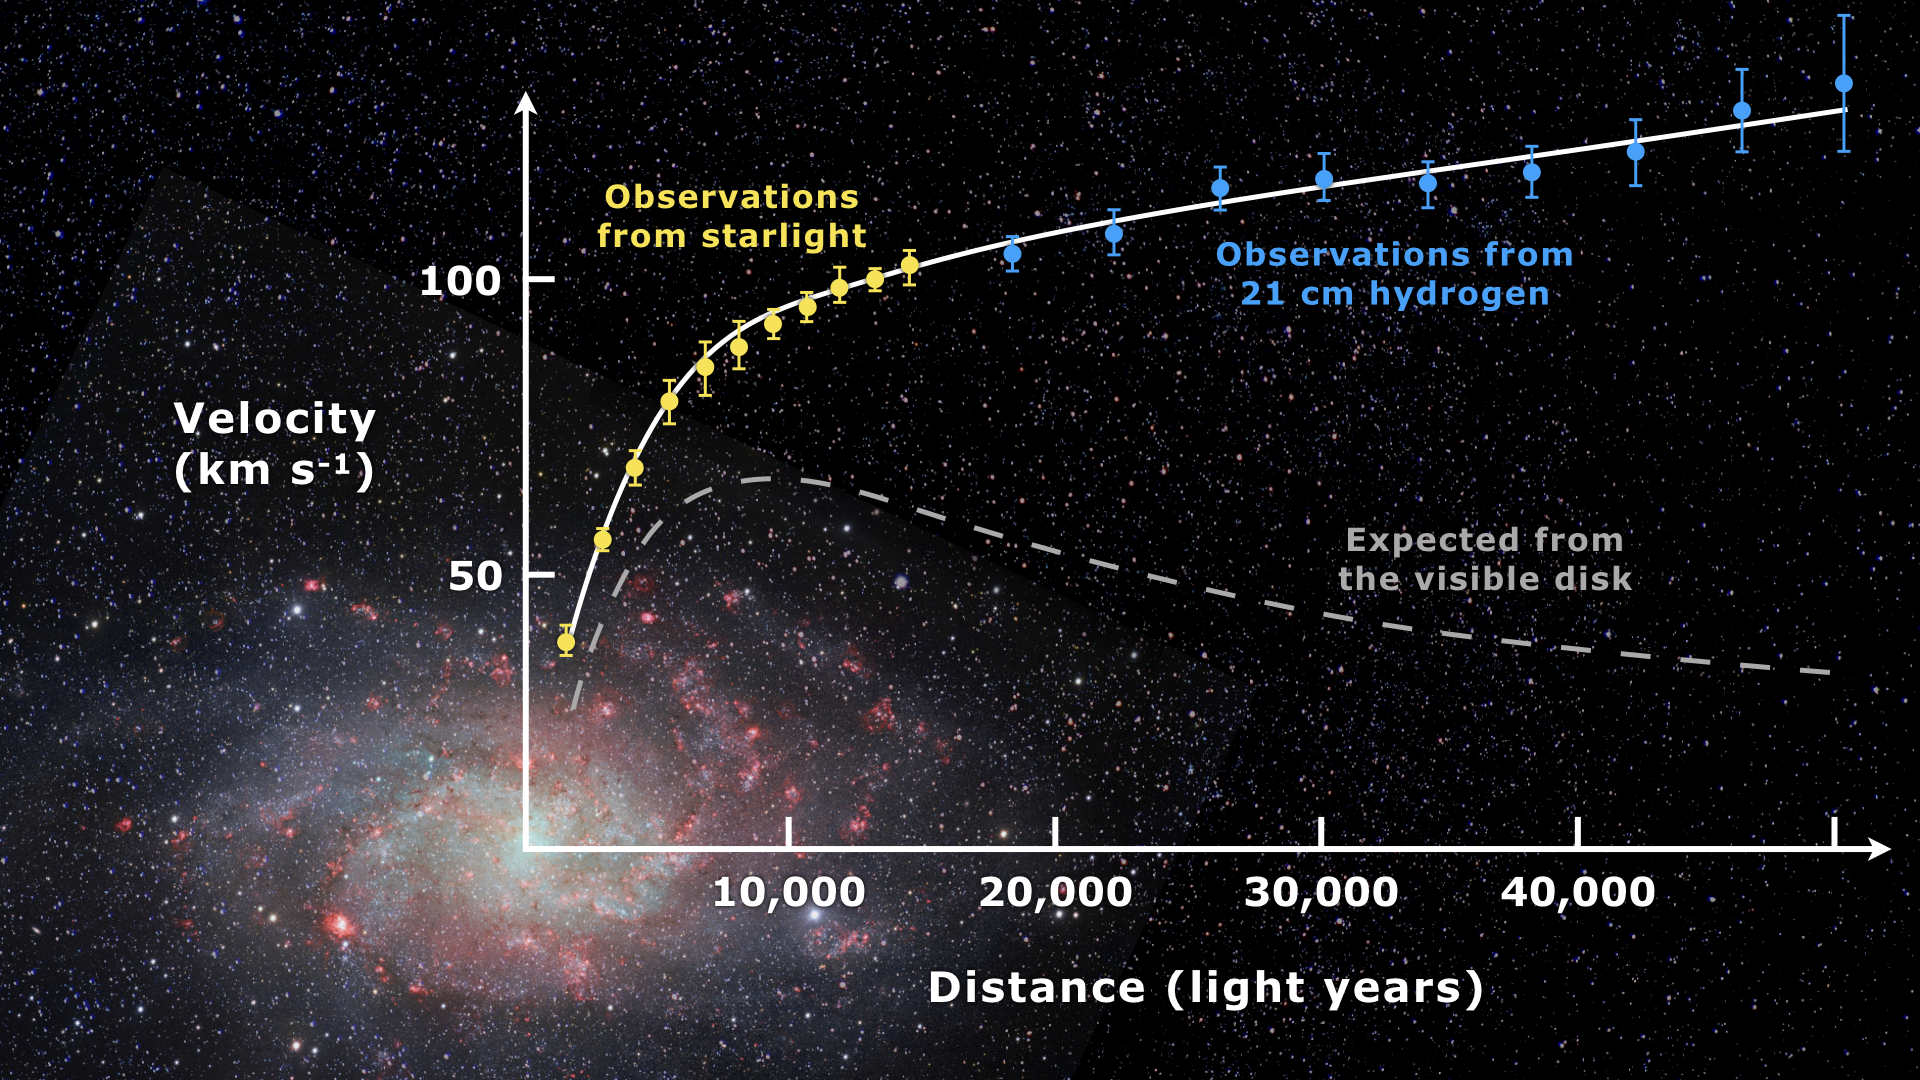
\includegraphics[width=\textwidth]{figures/rotation_curve.png}
   \caption[Rotation curve of Messier 33]{The rotation curve of the spiral galaxy Messier 33, adapted by Mario De Leo from measurements in Ref.~\cite{Corbelli}. The dashed line shows the expected velocity distribution using only the visible stars, demonstrating clear deviation from the observed velocities in both shape and magnitude which could be explained by the presence of a dark matter halo.}
   \label{fig:rotCurve}	
\end{figure}

The strong motivation for a particle explanation of dark matter has lead to an extremely broad scientific program to search for its interaction in high-energy physics experiments. 
While the mass density and distribution of dark matter is well constrained, almost nothing is currently known about its origins, particle mass, or non-gravitational interactions.
Potential dark matter particle candidates cover an extremely wide range of masses, from \SI{e-22}{\eV}, where the de Broglie wavelength of dark matter becomes too large to produce the observed galactic structure, to $\sim$5 solar masses, where stellar structures within dark matter halos would have visible tidal disruptions~\cite{rodriguez_2014}.
To help narrow the range of potential signals to search for, several classes of dark matter are defined which have promising features beyond reproducing the correct astronomical observations. 

Among these dark matter models is `light' dark matter, where dark matter may interact with standard model particles via kinetic mixing with the electromagnetic force~\cite{darkSectors}. 
This type of interaction would allow dark matter to be initially produced via interactions of SM particles and kept in thermal equilibrium with the early universe by interactions in the quark-gluon plasma.
As the universe expands and cools, the rate of dark matter production and annihilation would eventually slow below the expansion rate of the universe, stopping both its annihilation and production modes causing dark matter to `freeze-out' and leave behind a `relic' density observed today.

Through the requirements set by matching the relic density to the dark matter interaction rate, thermal relic models produce target mixing strengths for any given dark matter mass, creating useful experimental goals to set what scale of interaction needs to be searched for.
A basic kinetic mixing can be introduced by adding a new gauge boson, a type of particle which mediates interactions, which couples to the standard model hypercharge field with some mixing parameter and additionally interacts with some stable dark matter particle.
If this type of kinetic mixing were to exist, then physics interactions which produce standard model photons could instead very rarely produce this new massive gauge boson, referred to as a `Dark photon', or A'~\cite{Bauer_2018}. 

In this thesis, a search for a dark-photon-like signal is performed by selecting for `disappearing' muons in the compact muon solenoid (CMS) experiment. 
Produced frequently in high-energy collisions, muons are particles with nearly identical properties as electrons but with a much larger mass ($\sim$100 MeV compared to the electron mass of $\sim$0.5 MeV).
As muons pass through materials, they can interact with atomic nuclei and emit photons through a process known as `Bremsstrahlung'~\cite{tsai_1974}.

If Bremsstrahlung were to occur with a dark photon instead of a photon, the emitted \aprime would be kinematically favored to carry most of the incoming muon momentum.
As the A' would appear invisible to our detector, this interaction could result in the muon `disappearing', where a visible muon track with high energy suddenly stops without excess energy deposits nearby.
By measuring the rate that muons disappear within the detector, the frequency of this potential interaction and thus the amplitude of potential mixing between light dark matter and standard model matter can be constrained.

By looking for new physics interactions between muons and the detector itself, the CMS detector is used as a `fixed target' experiment rather than the standard collision experiment.
This poses several unique challenges for the analysis.
Muons must be identified with reduced detector information, as the target signal process will modify their behavior and break assumptions used in the standard particle reconstruction algorithms.
Additionally, rather than simulating the new physics process in an external event generator and importing it into the detector simulation it must be directly written into the simulation of the detector response, with the ability to calculate the total and differential cross section in a variety of materials over a range of incident muon energies to accurately simulate the interaction for any given muon.

To accomplish these goals, this search aims to select muons which originate from Z-bosons produced in the initial collision, which can produce two opposite-sign muons which peak strongly in invariant mass near \SI{91}{\giga\eV}.
Using the muon pairs produced in these decays, one muon can tag the event as a likely Z boson, and the other can be extrapolated into the detector to search for potential energy loss.
Because the probability of a fixed target interaction occurring is proportional to the amount of material traversed, we focus on muons passing through the CMS hadronic calorimeter, which forms the thickest part of the detector able to measure and reject potential SM interactions.

Signal events are categorized into two regions based on their behavior in the muon systems, which make up the outermost part of the CMS detector. 
Events with no reconstructed muons nearby are classified as `complete disappearance', while those with large energy differences between the probe track and the muon chamber track are classified as `partial disappearance' events.
Final measurements of the interaction rate are made by measuring the number of events that fall into these two signal regions, as well as the number of candidate probe tracks that are observed.
This rate is then combined with the thickness of the detector determined from simulation to interpret the rate in terms of a coupling strength, and the compatibilities of the number of measured interactions with only SM physics and with an added dark matter interaction are calculated.

%%%%%%%%%%%%%%%%%%%%%%%%%%%%%%%%%%%%%%%%%%%%%%%%%%%%%%%%%%%%%%%%%%%%%%%%%%%%%%%%
